\section{Warteschlange-Funktion für die Webcam}
Bei der Webcam\footnote{\url{https://dev.wetter-arbon.ch/webcam}} der Wetterstation handelt es sich um eine dreh-, schwenk- und zoombare Netzwerk-Kamera der Firma AXIS (Datenblatt siehe Anhang\,\ref{Spec_Webcam}). Die Webseite bietet die Möglichkeit die Webcam über den Browser zu steuern (pink hervorgehoben in Abbildung\,\ref{img:warteschlange}). Die Befehle an die Kamera werden dabei sequenziell abgearbeitet d.h. sind mehrere Nutzer gleichzeitig auf der Seite können sie sich gegenseitig beim Navigieren stören. Um dies zu verhindern wurde eine Warteschlange-Funktion hinzugefügt. Im Folgenden wird das Prinzip und die Umsetzung der Warteschlange erklärt.

%% ############################################################################
%% Unterkapitel
%% ############################################################################
\subsection{GUI der Warteschlange}
Jeder Benutzer, der die Webcam bedienen möchte, muss sich zuerst registrieren, indem er den Button \flqq Webcam bedienen\frqq drückt. Ist die Warteschlange leer erhält der Benutzer sofort Zugriff auf die Steuerung, was ihm mit einem grünen Balken und der verbleibenden Zeit signalisiert wird. Sind bereits andere Benutzer in der Warteschlange, so wird unterhalb des Buttons ein roter Balken mit der Wartezeit bis die Steuerung der Webcam freigegeben ist angezeigt (Abbildung\,\ref{img:warteschlange}, Mitte). Ist der Benutzer an der Reihe, hat er 40\,Sekunden Zeit die Webcam zu bedienen, bevor er sich neu registrieren muss. Die verbleibende Zeit wird wiederum im grünen Bereich unterhalb des Buttons angezeigt (siehe Abbildung\,\ref{img:warteschlange}, rechts).
\Diskussionspunkt{Warum 40 Sekunden?} \newline


\begin{figure}[htbp!]
  \fbox{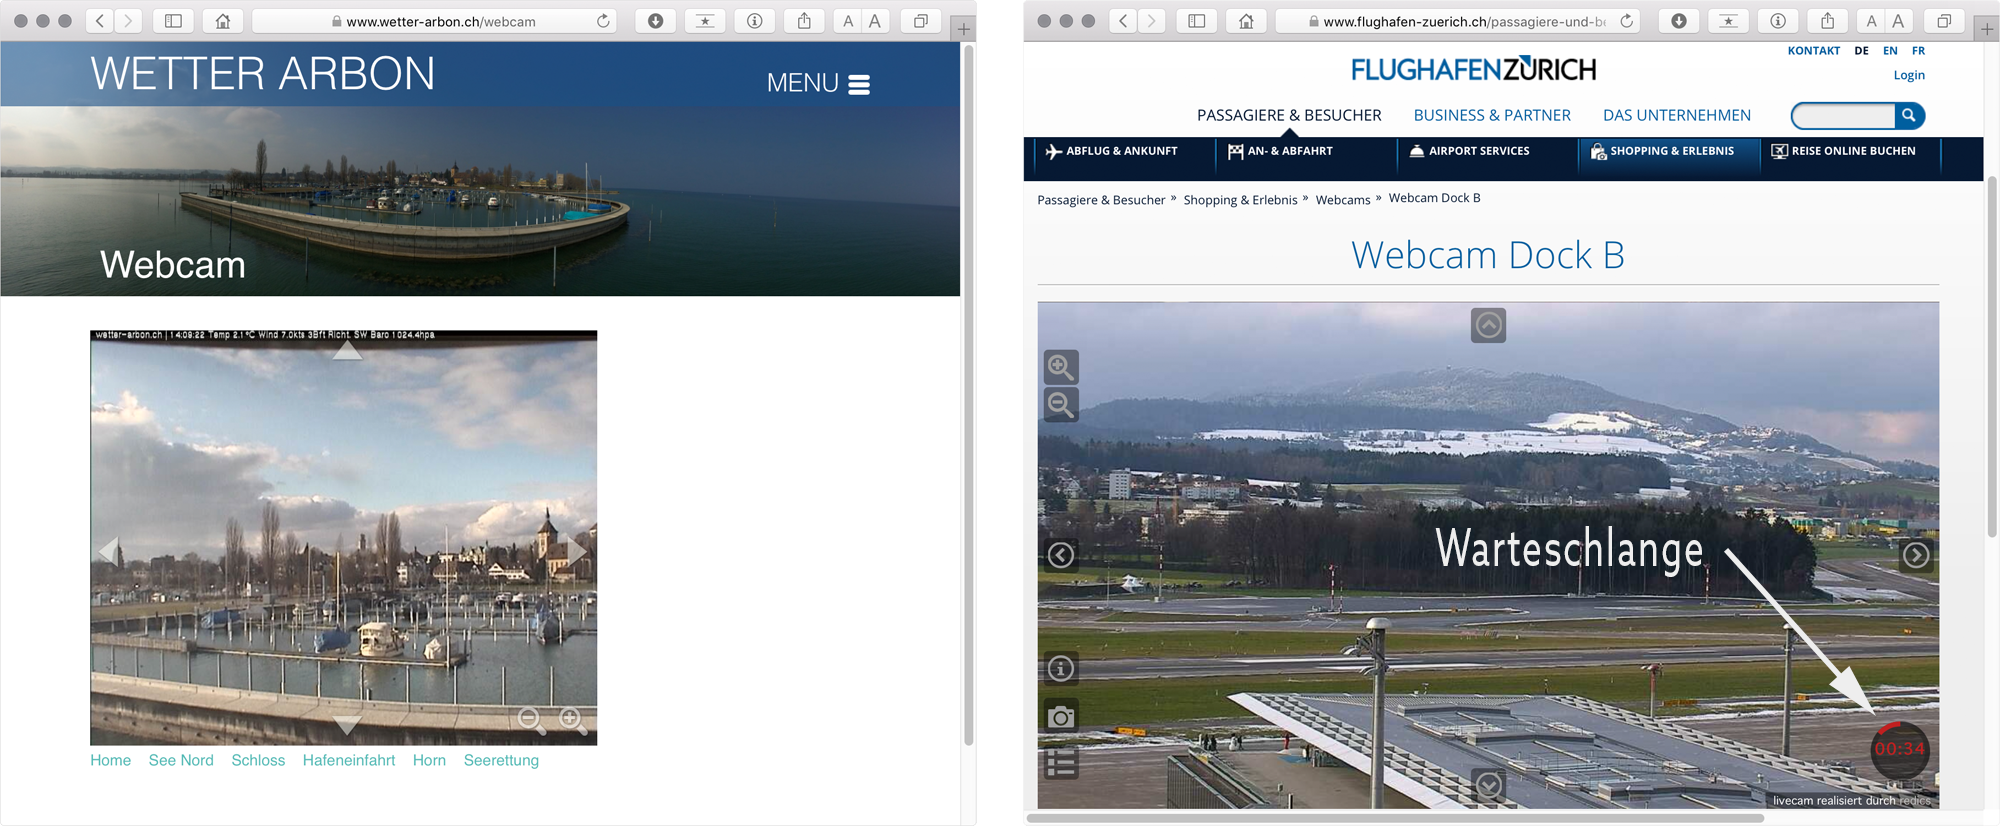
\includegraphics[width=\textwidth-2\fboxsep-2\fboxrule]{img/warteschlange.png}}
	\centering
	\caption{Darstellung der Warteschlange auf der Webseite}
	\label{img:warteschlange}
\end{figure}


%% ############################################################################
%% Unterkapitel
%% ############################################################################
\subsection{Technische Umsetzung der Warteschlange}
Die technische Umsetzung der Warteschlange ist vereinfacht in Abbildung\,\ref{img:warteschlangeprinzip} dargestellt. Registriert sich ein Benutzer per Klick auf den Registrierungsbutton wird eine Session-ID gelöst und diese per POST an den Server gesendet. Dieser prüft nun in der Datenbank ob bereits andere Benutzer in der Warteschlange sind und berechnet die Wartezeit (Beispiel in Listing\,\ref{lst:wartezeit}).

\begin{figure}[htbp!]
  \fbox{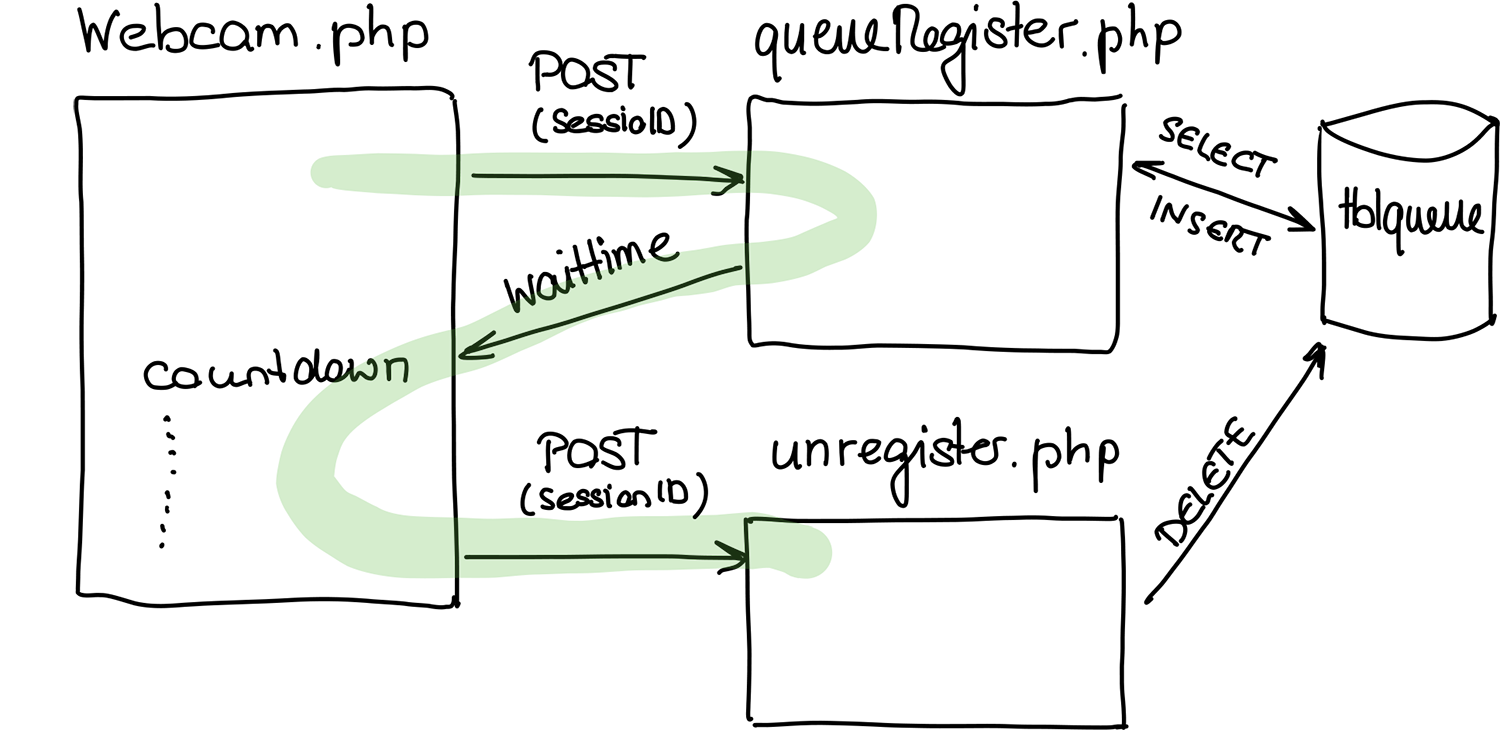
\includegraphics[width=\textwidth-2\fboxsep-2\fboxrule]{img/warteschlangeprinzip.png}}
	\centering
	\caption{Kommunikation zwischen Browser und Server}
	\label{img:warteschlangeprinzip}
\end{figure}

\noindent
Danach wird für den Benutzer einen Eintrag in der Tabelle erstellt (siehe Abbildung\,\ref{img:tblqueuemitBenutzer}), in dem steht wann sich der Benutzer registriert hat, wie lange seine Wartezeit ist und seine Session-ID. Zum Schluss sendet der Server dem Browser die berechnete Wartezeit.

\begin{figure}[htbp!]
  \fbox{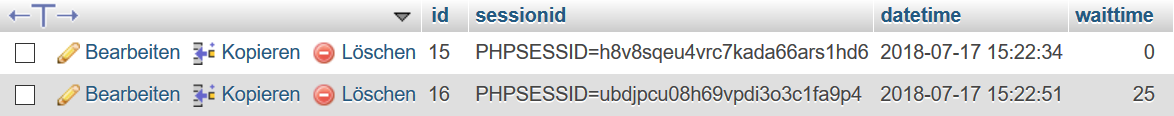
\includegraphics[width=\textwidth-2\fboxsep-2\fboxrule]{img/tblqueuemitBenutzer.png}}
	\centering
	\caption{Datenbankeintrag, mehrere Benutzer registriert sind}
	\label{img:tblqueuemitBenutzer}
\end{figure}

% Berechnung der Wartezeit
\begin{lstlisting}[label=lst:wartezeit, language=PHP, style=PHP]
$waittime = $waittimeVorgaenger + 40 - $abgelaufeneZeit +2;
// 0 + 40 - (51-34) + 2 = 25
\end{lstlisting}


\noindent
Eine Countdown-Funktion im Browser prüft nun selbständig wann die Wartezeit vorüber ist und gibt die Steuerung der Webcam frei. Die Freigabe funktioniert über eine einfache if-Bedingung, wo geprüft wird, ob der Browser registriert ist und die Wartezeit abgelaufen ist. Die if-Schleife ist in Listing\,\ref{lst:webcamControl} dargestellt.
Sobald die 40\,Sekunden Bedienzeit vorüber sind sendet der Browser wieder einen POST mit der Session-ID an den Server, welcher daraufhin den Eintrag in der Datenbank löscht. Wenn der Benutzer probiert die Webcam zu bedienen, ohne dass er sich registriert hat bzw. ohne dass er an der Reihe ist, wird ihm eine entsprechende Meldung angezeigt, wie in Listing\,\ref{lst:webcamControl} ersichtlich.

\begin{lstlisting}[label=lst:webcamControl, language=Python, style=py]
$('#webcam_up.on('click', function() {
  if(controlboolean == true && registerboolean == true)
    .....  // Kamera steuern moeglich
  else if (registerboolean == false){
    $("#countdown").html("Registiere dich fuer die Warteschlange um die Kamera zu bedienen");}
  else {
    $("#countdown").html("Habe Geduld du bist gleich an der Reihe");}
}
\end{lstlisting}


\begin{itemize}
\item \Diskussionspunkt{Für was wird die Session-ID benötigt? Als Zufallszahl um den DB-Eintrag löschen zu können?}
\item \Diskussionspunkt{Warum werden zwei verschiedene URL verwendet, wenn über action regsiter bzw. unregister unterschieden werden könnte?}
\item \Diskussionspunkt{Automatische Löschung wäre sinnvoller}
\item \Diskussionspunkt{Was wird gegen SQL-Injektion im Feld SID unternommen? Es ist keine escape-Funktion vorhanden }
\item \Diskussionspunkt{was passiert wenn der Benutzer das Browser-Fenster schliesst?}
\item \Diskussionspunkt{wie werden alte Einträge gelöscht?}
\item \Diskussionspunkt{DB-Abbildung mit mindestens drei Einträgen ist anschaulicher}
\end{itemize}
